\documentclass[epsfig,10pt,fullpage]{article} \addtolength{\textwidth}{1.5in}
\addtolength{\oddsidemargin}{-0.75in}
\addtolength{\topmargin}{-0.75in}
\addtolength{\textheight}{1.5in}
\addtolength{\evensidemargin}{0.75in}
\raggedbottom
\usepackage{ae,aecompl}
\usepackage{epsfig,float,times}
\usepackage{graphicx}
\usepackage[usenames]{xcolor}

\newcommand{\red}[1]{{\color{red}\sf{#1}}}
\newcommand{\blue}[1]{{\color{blue}\sf{#1}}}

\definecolor{AppleGreen}{rgb}{0.55, 0.71, 0.0}
\newcommand{\green}[1]{{\color{AppleGreen}\sf{#1}}}

\definecolor{Brass}{rgb}{0.71, 0.4, 0.11}

\usepackage{placeins}
\usepackage{listings}
\definecolor{PineGreen}{rgb}{0.0, 0.47, 0.44}
\lstset{
%language = C,
%language = Verilog,
basicstyle=\small\color{black}\ttfamily, commentstyle=\small\color{PineGreen}\itshape\ttfamily,
keywordstyle=\small\color{blue}\bfseries\ttfamily,
showstringspaces=false,
frame=none, %lines % boxed listings
breaklines=true,
breakatwhitespace=true,
tabsize=3
}

\begin{document}
~\\
\centerline{\huge Using the {\it DESim} Application with Verilog Code}
~\\
~\\
This tutorial introduces the {\it DESim} application, which you can use to simulate 
circuits specified with Verilog code. The {\it DESim} application provides a 
{\it graphical user interface} (GUI) that represents some of the features of a {\it DE1-SoC}
board. This GUI serves as a ``front end'' for the {\it ModelSim} simulator. Using the 
{\it DESim} GUI you can invoke both the ModelSim Verilog {\it compiler} and {\it simulator}. 
Inputs to the {\it ModelSim} simulator can be provided by clicking on features in the
{\it DESim} GUI, which also shows results produced by the simulator on displays that look
like the ones on a DE1-SoC board.

~\\
\noindent
{\bf Contents:}
\begin{itemize}
\item Getting Started with {\it DESim}
\item Compiling and Simulating {\it DESim} Sample Projects
\item Simulating a Circuit that Includes a Memory Module
\item Making a {\it DESim} Project
\item Troubleshooting Problems with the {\it DESim} Application
\end{itemize}

~\\
\noindent
{\bf Requirements:}
\begin{itemize}
\item A computer running Microsoft\textsuperscript{\textregistered} Windows\textsuperscript{\textregistered} (version 10 is recommended).
\item A good working knowledge of Verilog code.
\item ModelSim-Intel FPGA Starter Edition software, version 10.5b. This software must be
installed on the computer that is running the {\it DESim} software. The required
{\it ModelSim} software is part of the {\it Quartus Prime} suite of CAD tools provided by Intel\textsuperscript{\textregistered} Corporation. 
Version 10.5b of ModelSim is packaged with a number of {\it Quartus} software releases, including 
18.0, 18.1, and 19.0.
\item You should know how to use {\it ModelSim}\textsuperscript{\textregistered} to simulate Verilog code using a {\it testbench}. This material is presented in the tutorial {\it Using the 
ModelSim-Intel FPGA Simulator with Verilog Testbenches}.
\item The {\it DESim} application. Instructions for downloading and installing the {\it DESim} 
application are available in the document {\it Installing the DESim Application}, available from
the Intel FPGA Academic Program.
\end{itemize}

\section*{Getting Started}
Start the {\it DESim} program to reach the graphical user interface (GUI) shown in 
Figure~\ref{fig:gui}. You should see the message ``\green{The server is running...}'' at 
the top of the {\it message pane} in the GUI. If you do not see this message, but instead 
you see a message \red{Server setup failed}, then the {\it DESim} software is not working
properly and should be closed. In this case see the troubleshooting section at the end
of this document.

~\\
\noindent
On the right-hand side of Figure~\ref{fig:gui} the \texttt{LEDs} represent the 
red lights \red{\texttt{LEDR}$_{9-0}$} that are provided on a DE1-SoC board. The
\texttt{Switches} correspond to the board's \blue{\texttt{SW$_{9-0}$}} slide switches, the 
\texttt{Push Buttons} to \blue{\texttt{KEY$_{3-0}$}}, and the \texttt{Seven-segment
Displays} to \red{\texttt{HEX5}}, \red{\texttt{HEX4}}, $\cdots$, \red{\texttt{HEX0}}.
There are also some additional features in the GUI called \texttt{PS/2 Keyboard}, 
\texttt{Parallel Ports}, and \texttt{VGA Display}. These features of
the {\it DESim} GUI are not described in this document. 

~\\
\noindent
The {\it DESim} tool works in the context of a {\it project}. To introduce the features of the 
{\it DESim} GUI we will first open an existing project. This example is a multibit adder 
named {\it addern}, which is provided as a {\it demo} project along with the {\it DESim}
software. Referring to Figure~\ref{fig:gui}, click on the \texttt{Open Project} command 
to reach the dialogue displayed in Figure~\ref{fig:open}. As shown in the figure, navigate
to the \texttt{demos} folder, click to select the \texttt{addern} project, and then click the
\fbox{\texttt{Select Folder}} button.

\begin{figure}[t]
	\begin{center}
        \setlength{\fboxsep}{0pt}
        \fbox{\includegraphics[width = \textwidth]{figures/DESim_GUI.png}}
	\end{center}
		  \caption{The {\it DESim} GUI.}
	\label{fig:gui}
\end{figure}

\begin{figure}[t]
	\begin{center}
        \setlength{\fboxsep}{0pt}
        \fbox{\includegraphics[width = .9\textwidth]{figures/open_Addern.png}}
	\end{center}
		  \caption{Opening the {\it addern} project.}
	\label{fig:open}
\end{figure}
\clearpage
\newpage
\noindent
Using Microsoft Windows \texttt{File Explorer}, Figure~\ref{fig:project} shows the
contents of the file-system folder that holds the {\it addern} project. It consists of the 
folders named \texttt{sim} and \texttt{tb}, as well as the files called {\it Addern.v}, 
and {\it top.v}. There is also a {\it Readme.txt} file, but it just provides 
documentation and is not really a part of the {\it DESim} project. 

~\\
\begin{figure}[h]
	\begin{center}
        \setlength{\fboxsep}{0pt}
        \fbox{\includegraphics[width = .9\textwidth]{figures/project_Addern.png}}
	\end{center}
		  \caption{The {\it addern} folder.}
	\label{fig:project}
\end{figure}

~\\
\noindent
The {\it Addern.v} file, shown in Figure~\ref{fig:addern}, is the Verilog code that will 
be simulated in this part of the tutorial. We will use the {\it DESim} GUI to specify signal 
values for the adder's inputs, {\it Cin}, {\it X}, and {\it Y}, and then display the
simulation results produced for the outputs, {\it Sum} and {\it Cout}, on the \texttt{LEDs}. 
To make connections between the adder's ports and the signals that are associated with the
{\it DESim} GUI we {\it instantiate} the {\it Addern} module in another Verilog module
called {\it top}. This module is defined in the file {\it top.v}, displayed in 
Figure~\ref{fig:top}. Its ports use the signal names that are appropriate for a
top-level Verilog module which is intended to be implemented on a DE1-SoC board. These
port names include \texttt{CLOCK\_50}, \texttt{SW}, \texttt{KEY}, \texttt{HEX0}, $\cdots$,
\texttt{HEX5}, and  \texttt{LEDR}. For the {\it Addern} module we only use some of these ports,
and leave the others unconnected (the unused ports are included for consistency with other
{\it DESim} {\it demo} projects).

~\\
\noindent
The {\it Addern} module is instantiated in Line~\ref{line:U1} in {\it top.v} by the statement

\begin{lstlisting}[]
    Addern U1 (SW[9], SW[3:0], SW[7:4], LEDR[3:0], LEDR[4]);
\end{lstlisting}

~\\
\noindent
This statement connects the switch {\it SW}$_9$ to the multibit adder's carry-in, {\it Cin}, 
and it connects {\it SW}$_{3-0}$ and  {\it SW}$_{7-4}$ to the adder's {\it X} and {\it Y} 
data inputs, respectively.  The {\it Sum} output is attached to {\it LEDR}$_{3-0}$, and 
the carry-out, {\it Cout}, is connected to {\it LEDR}$_4$.

\lstset{language=Verilog,numbers=none,escapechar=|}
\begin{figure}[h]
\begin{center}
\begin{minipage}[t]{12.5 cm}
\begin{lstlisting}[name=addern]
// A multi-bit adder
module Addern (Cin, X, Y, Sum, Cout);
    parameter n = 4;
    input Cin;
    input [n-1:0] X, Y;
    output [n-1:0] Sum;
    output Cout;

    assign {Cout, Sum} = X + Y + Cin;
endmodule
\end{lstlisting}
\end{minipage}
\caption{Verilog code for the multibit adder.}
\label{fig:addern}
\end{center}
\end{figure}

\lstset{language=Verilog,numbers=left,escapechar=|}
\begin{figure}[h]
\begin{center}
\begin{minipage}[t]{14 cm}
\begin{lstlisting}[name=top]
module top (CLOCK_50, SW, KEY, LEDR, HEX0, HEX1, HEX2, HEX3, HEX4, HEX5);

    input CLOCK_50;             // DE-series 50 MHz clock signal
    input wire [9:0] SW;        // DE-series switches
    input wire [3:0] KEY;       // DE-series pushbuttons
    output wire [9:0] LEDR;     // DE-series LEDs   

    output wire [6:0] HEX0;     // DE-series HEX displays
    output wire [6:0] HEX1;
    output wire [6:0] HEX2;
    output wire [6:0] HEX3;
    output wire [6:0] HEX4;
    output wire [6:0] HEX5;

    |\label{line:U1}|Addern U1 (SW[9], SW[3:0], SW[7:4], LEDR[3:0], LEDR[4]);

endmodule
\end{lstlisting}
\end{minipage}
    \caption{Verilog code for the {\it top} module.}
\label{fig:top}
\end{center}
\end{figure}

~\\
\noindent
To compile the {\it addern} project, in the {\it DESim} GUI click the \texttt{Compile Testbench}
command. This command executes a {\it batch} file called {\it run\_compile.bat}, which is 
found in the \texttt{sim} folder of the {\it addern} project. This batch file comprises
some {\it ModelSim} commands, shown below:

\lstset{language=command.com,numbers=none,escapechar=|}
\begin{lstlisting}[]
    if exist work rmdir /S /Q work

    vlib work
    vlog ../tb/*.v
    vlog ../*.v
\end{lstlisting}

~\\
\noindent
The batch file executes the {\it vlib} command, which is part of the {\it ModelSim} software,
to create a \texttt{work} folder (first deleting this folder if it already exists). The batch file
then invokes the {\it ModelSim} Verilog compiler, {\it vlog}, twice. The first invocation
of the compiler, \texttt{vlog ../tb/*.v}, compiles the Verilog source code in the {\it addern}
project's \texttt{tb} folder. This folder holds the {\it testbench} for the project, which is
described shortly. The second call to {\it vlog} compiles the source-code of the 
{\it DESim} project, which includes the files {\it Addern.v} and {\it top.v}. Any messages
produced while executing {\it run\_compile.bat} are displayed inside the message pane in
the {\it DESim} GUI, as illustrated in Figure~\ref{fig:compile}.

\begin{figure}[t]
	\begin{center}
        \setlength{\fboxsep}{0pt}
        \fbox{\includegraphics[width = \textwidth]{figures/run_compile.png}}
	\end{center}
          \caption{Messages produced by executing {\it run\_compile.bat}.}
	\label{fig:compile}
\end{figure}
\newpage
~\\
\noindent
The testbench file for the {\it addern} project that is compiled by the command 
\texttt{vlog ../tb/*.v} is called {\it tb.v}, and is displayed in Figure~\ref{fig:tb}. 
It is not necessary to modify (or even examine) much of this code to use the {\it
DESim} software, but we describe some of the code here for completeness.
The testbench code in the figure has a general structure that 
allows it to be used to simulate different
examples of Verilog code that might be used in various {\it DESim} projects. Hence, not
all of the code in the testbench is needed for the {\it addern} project.  Line~\ref{line:tb} 
declares the testbench module, which is named {\it tb}. 
The next several lines in the code declare some signals that are used in the testbench. 
The statement

\lstset{language=Verilog,numbers=none,escapechar=|}
\begin{lstlisting}[]
    initial $sim_fpga(CLOCK_50, SW, KEY, LEDR, HEX, key_action, scan_code, 
                      ps2_lock_control, VGA_X, VGA_Y, VGA_COLOR, plot, GPIO);
\end{lstlisting}

~\\
\noindent
is unique to the {\it DESim} program. It makes use of a special feature of the {\it ModelSim}
software that allows communication with a {\it custom software function}. In this case
the custom function is part of the {\it DESim} software and is called {\it sim\_fpga}. 
This function is stored in a file named {\it simfpga.vpi}, which has to be included in 
the \texttt{sim} folder of each {\it DESim} project. The {\it DESim} GUI sends/receives signal 
values to/from the ModelSim software via the {\it sim\_fpga} function. 
This {\it ModelSim} capability is known as the {\it Verilog Procedural Interface} (VPI). 

\lstset{language=Verilog,numbers=left,escapechar=|}
\begin{figure}[H]
\begin{center}
\begin{minipage}[t]{15 cm}
\begin{lstlisting}[name=tb]
`timescale 1ns / 1ns
`default_nettype none

// This testbench is designed to hide the details of using the VPI code

|\label{line:tb}|module tb();

    reg CLOCK_50 = 0;               // DE-series 50 MHz clock
    reg [9:0] SW = 0;               // DE-series SW switches
    reg [3:0] KEY = 0;              // DE-series pushbutton keys
    wire [(8*6) -1:0] HEX;          // HEX displays (six ports)
    wire [9:0] LEDR;                // DE-series LEDs

    reg key_action = 0;
    reg [7:0] scan_code = 0;
    wire [2:0] ps2_lock_control;

    wire [7:0] VGA_X;               // "VGA" column
    wire [6:0] VGA_Y;               // "VGA" row
    wire [2:0] VGA_COLOR;           // "VGA pixel" colour (0-7)
    wire plot;                      // "Pixel" is drawn when this is pulsed
    wire [31:0] GPIO;               // DE-series GPIO port

    initial $sim_fpga(CLOCK_50, SW, KEY, LEDR, HEX, key_action, scan_code, 
                      ps2_lock_control, VGA_X, VGA_Y, VGA_COLOR, plot, GPIO);

    wire [6:0] HEX0;                // DE-series HEX0 port
    wire [6:0] HEX1;                // DE-series HEX1 port
    wire [6:0] HEX2;                // ...
    wire [6:0] HEX3;
    wire [6:0] HEX4;
    wire [6:0] HEX5;

    // create the 50 MHz clock signal
    always #10
        CLOCK_50 <= ~CLOCK_50;

    // connect the single HEX port on "sim_fpga" to the six DE-series HEX ports
    assign HEX[47:40] = {1'b0, HEX0};
    assign HEX[39:32] = {1'b0, HEX1};
    assign HEX[31:24] = {1'b0, HEX2};
    assign HEX[23:16] = {1'b0, HEX3};
    assign HEX[15: 8] = {1'b0, HEX4};
    assign HEX[ 7: 0] = {1'b0, HEX5};
    
    |\label{line:DUT}|top DUT (.CLOCK_50(CLOCK_50), .SW(SW), .LEDR(LEDR), .KEY(KEY), .HEX0(HEX0), 
             .HEX1(HEX1), .HEX2(HEX2), .HEX3(HEX3), .HEX4(HEX4), .HEX5(HEX5));

endmodule
\end{lstlisting}
\end{minipage}
        \caption{The testbench file, {\it tb.v}, for the {\it addern} project.}
\label{fig:tb}
\end{center}
\end{figure}

~\\
\noindent
Line~\ref{line:DUT} in the testbench code instantiates the 
{\it design under test} (DUT), which is the Verilog module named {\it top} shown in 
Figure~\ref{fig:top}. To execute the testbench using the {\it ModelSim} simulator, click on the
\texttt{Start Simulation} command in the {\it DESim} GUI. This command executes a {\it batch} file 
called {\it run\_sim.bat}, which is found in the \texttt{sim} folder of the 
{\it addern} project. This batch file runs {\it vsim}, the {\it ModelSim} Verilog
simulator, using the command:

~\\
\begin{minipage}[h]{17.5 cm}
\lstset{language=Verilog,numbers=none,escapechar=|}
\begin{lstlisting}[]
vsim -pli simfpga.vpi -Lf 220model -Lf altera_mf_ver -Lf verilog -c -do "run -all" tb
\end{lstlisting}
\end{minipage}

~\\
\noindent
The \texttt{-pli} argument for the {\it vsim} program instructs it to link to the
{\it sim\_fpga} software function that has been (previously) compiled into the 
{\it simpfga.vpi} file. The \texttt{-L} arguments include some simulation libraries for
Intel FPGAs that may be needed by the simulator. Finally, the remaining arguments 
run the simulation for the top-level module, which is {\it tb}. Any messages 
produced while executing {\it run\_sim.bat} are displayed inside the message pane in
the {\it DESim} GUI, as depicted in Figure~\ref{fig:sim}.

~\\
\noindent
As mentioned previously, the {\it addern} project includes a {\it Readme.txt} file that
documents its usage. This file is displayed in Figure~\ref{fig:readme}. You can follow
its instructions to see how the switches and lights are used for the project (of course, 
you can also find this information by looking at the Verilog source code). An example
simulation result is illustrated in Figure~\ref{fig:sim}. It corresponds to {\it Cin} $= 1$,
$X = (0110)_2 = (6)_{10}$, and $Y = (1010)_2 = (10)_{10}$. The result of the addition is
$(10001)_2 = (17)_{10}$ ({\it Cout} $= 1$, with {\it Sum} $= (0001)_2$), which is displayed on 
the \texttt{LEDs}.  Try different settings for the
\texttt{SW} switches and observe the results displayed on the \texttt{LEDs}.

~\\
~\\
\begin{figure}[h]
	\begin{center}
        \setlength{\fboxsep}{0pt}
        \fbox{\includegraphics[width = \textwidth]{figures/run_simulation.png}}
	\end{center}
          \caption{Messages produced by executing {\it run\_sim.bat}.}
	\label{fig:sim}
\end{figure}

\lstset{language=make,numbers=none,escapechar=|}
\begin{figure}[h]
\begin{center}
\begin{minipage}[t]{12.5 cm}
\begin{lstlisting}[name=top]
To use this demo:

-- set a value, X, using SW[3:0]
-- set a value, Y, using SW[7:4]
-- set a carry-in, Cin, using SW[9]

The circuit produces the 5-bit Sum = X + Y + Cin,
which is displayed on LED[4:0]
\end{lstlisting}
\end{minipage}
    \caption{The {\it Readme.txt} file for the {\it addern} project.}
\label{fig:readme}
\end{center}
\end{figure}

~\\
\noindent
We have now finished discussing the {\it addern} sample project.

\section*{Simulating a Sequential Circuit}

Another {\it DESim} sample project called {\it counter} is included in the {\it DESim}
\texttt{demos} folder. Use the \texttt{Open Project} command in the {\it DESim} GUI to open this
project. As illustrated in Figure~\ref{fig:project2} using \texttt{File Explorer}, the
contents of the file-system folder for this project look the same as for the 
{\it addern} project (Figure~\ref{fig:project}), except that there is a Verilog
source-code file named {\it Counter.v}. Figure~\ref{fig:counter}
shows the contents of the {\it Counter.v} file. It represents a 24-bit counter with synchronous
reset. The port names for this module correspond to the signal names 
on the DE1-SoC board, with {\it KEY}$_0$ being used for reset, {\it CLOCK\_50} for the 
clock signal, and {\it LEDR} for the outputs. Since {\it LEDR} is a 10-bit signal and the 
counter has 24 bits, only a subset of the counter outputs (the most-significant ones) are 
connected to {\it LEDR}. 

~\\
\begin{figure}[h]
	\begin{center}
        \setlength{\fboxsep}{0pt}
        \fbox{\includegraphics[width = .9\textwidth]{figures/project_Counter.png}}
	\end{center}
		  \caption{The {\it counter} folder.}
	\label{fig:project2}
\end{figure}

\lstset{language=Verilog,numbers=none,escapechar=?}
\begin{figure}[h]
\begin{center}
\begin{minipage}[t]{12.5 cm}
\begin{lstlisting}[name=accumulate]
module Counter (KEY, CLOCK_50, LEDR);
    input [0:0] KEY;
    input CLOCK_50;
    output [9:0] LEDR;
    parameter n = 24;
   
    reg [n-1:0] Count;
    wire Clock, Resetn;

    assign Clock = CLOCK_50;
    assign Resetn = KEY[0];

    // the counter
    always @(posedge Clock)
        if (Resetn  == 1'b0)        // synchronous clear
            Count <= 0;
        else
            Count <= Count + 1;

    assign LEDR = Count[n-1:n-10];
endmodule
\end{lstlisting}
\end{minipage}
\caption{Verilog code for the 24-bit counter.}
\label{fig:counter}
\end{center}
\end{figure}

~\\
\noindent
As described for the {\it addern} project, the {\it Counter} module is {\it instantiated}
in another Verilog module called {\it top}. This module is displayed in 
Figure~\ref{fig:top2}. It is the same as the one from Figure~\ref{fig:top}, except that 
Line~\ref{line:U1_counter} instantiates the {\it Counter} module.
The port \texttt{KEY[0]} in the \texttt{top}
module is connected to the counter's reset input, \texttt{CLOCK\_50} to its clock input, 
and \texttt{LEDR} to the counter's output port. 

~\\
\noindent
To compile the {\it counter} project, in the {\it DESim} GUI click the \texttt{Compile Testbench}
command. This command executes the {\it batch} file called {\it run\_compile.bat}, which
is found in the \texttt{sim} folder of the {\it counter} project. This batch file 
is identical to the one described earlier for the {\it addern} project. 
The testbench file that is compiled by {\it run\_compile.bat} for the {\it counter} project is  
found in its \texttt{tb} folder. This testbench, {\it tb.v}, is identical to the one shown 
in Figure~\ref{fig:tb}.

~\\
To execute the testbench for the {\it counter} project, click on the
\texttt{Start Simulation} command in the {\it DESim} GUI. This command executes the
{\it batch} file called {\it run\_sim.bat}. It is identical the one described for the 
{\it addern} project and runs the {\it vsim} Verilog simulator.

~\\
\lstset{language=Verilog,numbers=left,escapechar=|}
\begin{figure}[H]
\begin{center}
\begin{minipage}[t]{14 cm}
\begin{lstlisting}[name=top2]
module top (CLOCK_50, SW, KEY, LEDR, HEX0, HEX1, HEX2, HEX3, HEX4, HEX5);

    input CLOCK_50;             // DE-series 50 MHz clock signal
    input wire [9:0] SW;        // DE-series switches
    input wire [3:0] KEY;       // DE-series pushbuttons
    output wire [9:0] LEDR;     // DE-series LEDs   

    output wire [6:0] HEX0;     // DE-series HEX displays
    output wire [6:0] HEX1;
    output wire [6:0] HEX2;
    output wire [6:0] HEX3;
    output wire [6:0] HEX4;
    output wire [6:0] HEX5;

    |\label{line:U1_counter}|Counter U1 (KEY[0], CLOCK_50, LEDR);

endmodule
\end{lstlisting}
\end{minipage}
        \caption{The {\it top} module for the {\it counter} project.}
\label{fig:top2}
\end{center}
\end{figure}
\newpage
\noindent
The {\it Readme.txt} file for the {\it counter} project specifies:

\lstset{language=make,numbers=none,escapechar=|}
\begin{lstlisting}[]
To use this demo, reset the circuit by pressing and releasing KEY[0].
\end{lstlisting}

~\\
In the {\it DESim} GUI when the \texttt{Push Buttons} have a check mark shown, they are set to the
value 1. To reset the counter circuit, click \texttt{KEY}$_0$ once to {\it press} this button
(this action sets the corresponding signal for this button to 0), and then click it again
to {\it release} the button. The 24-bit counter will start to operate and the ten
most-significant counter outputs will be displayed on the \texttt{LEDs}. A screen-shot of
the {\it DESim} GUI while simulating the {\it counter} project is shown in 
Figure~\ref{fig:sim2}.

~\\
\begin{figure}[h]
	\begin{center}
        \setlength{\fboxsep}{0pt}
        \fbox{\includegraphics[width = \textwidth]{figures/run_simulation2.png}}
	\end{center}
          \caption{Simulating the {\it counter} project.}
	\label{fig:sim2}
\end{figure}

\newpage
\section*{Simulating a Circuit that Includes a Memory Module}

The {\it DESim} \texttt{demos} folder includes a project called {\it display}. It shows how 
to instantiate a memory module in Verilog code, and how to initialize the stored contents of 
the memory in a {\it DESim} simulation.  Use the \texttt{Open Project} command to open this
example project. As illustrated in Figure~\ref{fig:project3}, the
contents of the file-system folder for this project look similar to the previous ones,
but there are two extra files: {\it inst\_mem.v} and {\it inst\_mem.mif}. These files are
used for the memory module in the circuit, which is described shortly.

~\\
\begin{figure}[h]
	\begin{center}
        \setlength{\fboxsep}{0pt}
        \fbox{\includegraphics[width = .9\textwidth]{figures/project_Display.png}}
	\end{center}
		  \caption{The {\it display} folder.}
	\label{fig:project3}
\end{figure}

~\\
Figure~\ref{fig:display} shows the Verilog code for {\it Display.v}, which 
has ports named {\it KEY}, {\it SW}, {\it HEX0}, and {\it LEDR}.
Figure~\ref{fig:memory}$a$ gives a logic circuit that corresponds to the code in 
Figure~\ref{fig:display}. The circuit contains a counter that is used to read the 
contents of successive locations in a memory. This memory provides codes in ASCII format 
for some upper- and lower-case letters, which are provided as inputs to a decoder module. 
The counter and memory modules have a common clock signal, and the counter has a
synchronous clear input. Each successive clock cycle advances the counter and reads 
a new ASCII code from the memory. Since the counter is three-bits wide, only the first 
eight locations in the memory are read (the upper two address bits on the memory are set
to 00), and they provide the ASCII codes for letters A, b, C, d, E, F, g, and h. The 
decoder produces an appropriate bit-pattern to render each letter on a seven-segment display.

~\\
\noindent
The memory used in the logic circuit is depicted in part $b$ of Figure~\ref{fig:memory}. It
is a $32 \times 8$ synchronous read-only memory (ROM), which has a register for holding 
address values. The memory is specified in the Verilog file {\it inst\_mem.v}, and it is 
initialized with the contents of the file {\it inst\_mem.mif},
which is illustrated in Figure~\ref{fig:mif}. This file contains the ASCII codes for the 
eight letters displayed by the circuit.

\lstset{language=Verilog,numbers=none,escapechar=?}
\begin{figure}[h!]
\begin{center}
\begin{minipage}[t]{15 cm}
\begin{lstlisting}[name=display]
module Display (KEY, SW, HEX0, LEDR);
    input [0:0] KEY;
    input [0:0] SW;
    output reg [6:0] HEX0;
    output [9:0] LEDR;	

    parameter A = 8'd65, b = 8'd98, C = 8'd67, d = 8'd100, E = 8'd69, 
        F = 8'd70, g = 8'd103, h = 8'd104;
    wire Resetn, Clock;
    wire [2:0] Count;
    wire [7:0] char;

    assign Resetn = SW[0];
    assign Clock = KEY[0];

    count3 U1 (Resetn, Clock, Count);
    inst_mem U2 ({2'b0, Count}, Clock, char);
    assign LEDR = {2'b0, char};

    always @(*)
        case (char)
            A: HEX0 = 7'b0001000;
            b: HEX0 = 7'b0000011;
            C: HEX0 = 7'b1000110;
            d: HEX0 = 7'b0100001;
            E: HEX0 = 7'b0000110;
            F: HEX0 = 7'b0001110;
            g: HEX0 = 7'b0010000;
            h: HEX0 = 7'b0001011;
            default HEX0 = 7'b1111111;
        endcase
endmodule

module count3 (Resetn, Clock, Q);
    input Resetn, Clock;
    output reg [2:0] Q;

    always @ (posedge Clock)
        if (Resetn == 0)
            Q <= 3'b000;
        else
            Q <= Q + 1'b1;
endmodule
\end{lstlisting}
\end{minipage}
        \caption{Verilog code for the {\it display} project.}
\label{fig:display}
\end{center}
\end{figure}

\begin{figure}[t]
	\begin{center}
		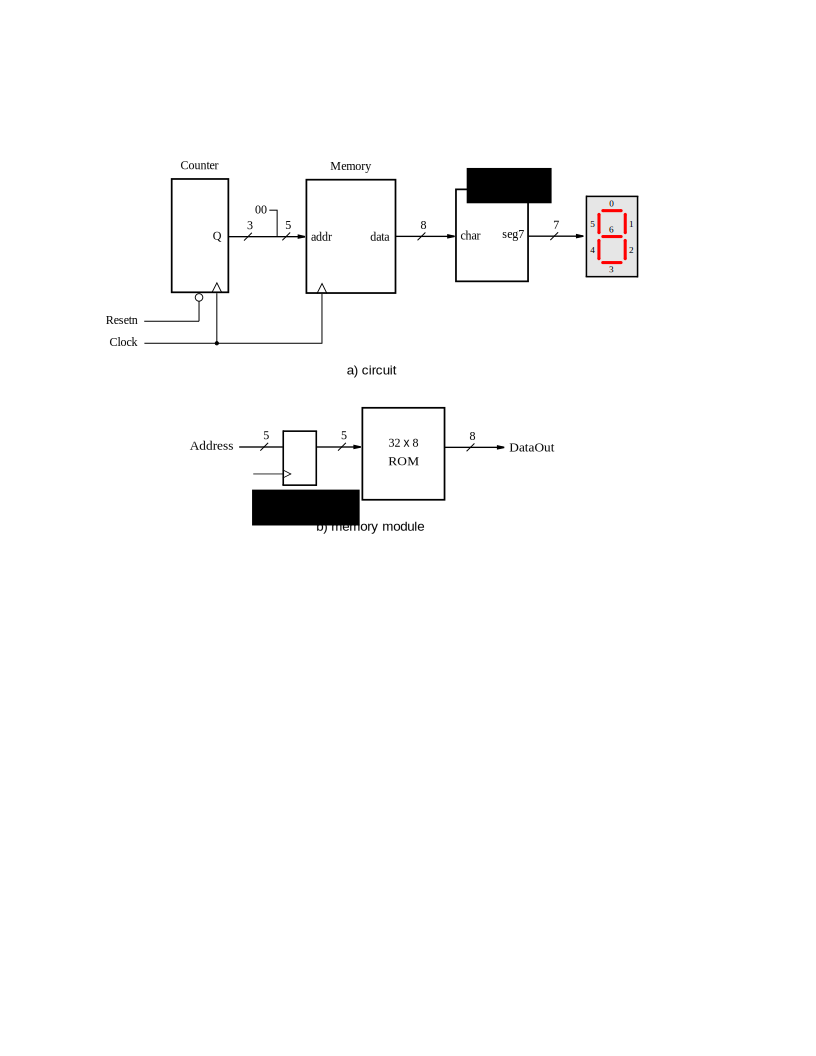
\includegraphics[scale = 1.0]{figures/figdisplay.pdf}
	\end{center}
          \caption{A circuit that represents the {\it display} project.}
	\label{fig:memory}
\end{figure}

~\\
\begin{figure}[bh!]
\begin{center}
\begin{minipage}[t]{12.5 cm}
\begin{tabbing}
DEPTH = 32;\\
WIDTH = 8;\\
ADDRESS\_RADIX = HEX;\\
DATA\_RADIX = DEC;\\
CONTENT\\
BEGIN\\
BEGI\=00X\=: \=104;XXXX\=\% A \=\% \kill
\>00 \>: \>65;    \>\% A \>\%\\
\>01 \>: \>98;    \>\% b \>\%\\
\>02 \>: \>67;    \>\% C \>\%\\
\>03 \>: \>100;   \>\% d \>\%\\
\>04 \>: \>69;    \>\% E \>\%\\
\>05 \>: \>70;    \>\% F \>\%\\
\>06 \>: \>103;   \>\% g \>\%\\
\>07 \>: \>104;   \>\% h \>\%\\
END;
\end{tabbing}
\end{minipage}
\end{center}
    \caption{The {\it inst\_mem.mif} memory initialization file.}
\label{fig:mif}
\end{figure}

\clearpage
\newpage
\noindent
To compile the {\it display} project, in the {\it DESim} GUI click the \texttt{Compile Testbench}
command. This command executes the project's {\it run\_compile.bat} script, which
is in its \texttt{sim} folder. This batch file is shown below:

\begin{center}
\begin{minipage}[h]{12.5 cm}
\lstset{language=command.com,numbers=left,escapechar=|}
\begin{lstlisting}[]
    |\label{line:bat1}|if exist ..\inst_mem.mif (
        copy /Y ..\inst_mem.mif .
    |\label{line:bat2}|)
    |\label{line:bat3}|if exist ..\inst_mem_bb.v (
        del ..\inst_mem_bb.v
    |\label{line:bat4}|)
    if exist work rmdir /S /Q work

    vlib work
    vlog ../tb/*.v
    vlog ../*.v
\end{lstlisting}
\end{minipage}
\end{center}

\noindent
Lines \ref{line:bat1} to \ref{line:bat2} are used to copy the memory initialization file,
{\it inst\_mem.mif}, from the \texttt{display} project folder into the \texttt{sim}
folder. This is done for two reasons: 1. {\it ModelSim} requires the file to be in the
\texttt{sim} folder to properly initialize the memory module during a simulation, and 2. 
if the file is changed in the \texttt{display} folder, then the latest version of the file 
will always be used when starting a simulation. Lines~\ref{line:bat3} to \ref{line:bat4}
delete a file called {\it inst\_mem\_bb.mif} that is sometimes associated with a memory
module; if present, this file would cause a {\it ModelSim} error. The rest of the batch
file, which compiles the Verilog code, is the same as for the previously-described {\it DESim}
projects.

~\\
\noindent
The testbench file {\it tb.v} that is compiled by {\it run\_compile.bat} for the {\it display}
project is identical to the one used for the {\it addern} project, shown in Figure~\ref{fig:tb}.
To execute the testbench for the {\it display} project, click on 
\texttt{Start Simulation}. Its {\it run\_sim.bat} script is the same as the 
ones used for the {\it addern} and {\it counter} projects.

~\\
The {\it Readme.txt} file for the {\it display} project is shown in Figure~\ref{fig:readme2}.
You can follow its instructions to read successive locations out of the memory and
display the corresponding characters on \texttt{HEX0}. An example simulation output after
first resetting the circuit and then creating a few clock cycles using \texttt{KEY[0]}
is illustrated in Figure~\ref{fig:sim3}.

\lstset{language=make,numbers=none,escapechar=|}
\begin{figure}[h]
\begin{center}
\begin{minipage}[t]{12.5 cm}
\begin{lstlisting}[name=top]
To use this demo:

-- The clock input is created by toggling KEY[0]
-- The active-low synchronous reset input is SW[0]

The circuit displays "characters" stored in a ROM on HEX0.
To use the circuit:

1. Set SW[0] to 0 to allow the circuit to be reset
2. pulse KEY[0] down/up to make a clock cycle
    -- the character 'A', the first character stored
	    in the ROM should be displayed on HEX0 
3. Set SW[0] to 1 so that the reset is not active
4. pulse KEY[0] down/up to make a clock cycle
5. pulse KEY[0] down/up to make a clock cycle
    -- HEX0 should now show 'b', the next character 
	    stored in the ROM
6. pulse KEY[0] down/up to make a clock cycle
    -- HEX0 should now show 'C', the next character 
	    stored in the ROM
7. etc (there are eight characters stored in the ROM)
\end{lstlisting}
\end{minipage}
    \caption{The {\it Readme.txt} file for the {\it display} project.}
\label{fig:readme2}
\end{center}
\end{figure}

\begin{figure}[t]
	\begin{center}
        \setlength{\fboxsep}{0pt}
        \fbox{\includegraphics[width = \textwidth]{figures/run_simulation3.png}}
	\end{center}
          \caption{Simulating the {\it display} project.}
	\label{fig:sim3}
\end{figure}

\section*{Setting up a {\it DESim} Project}

An easy way to set up your own {\it DESim} project is to use one of the example projects in
the {\it DESim} \texttt{demos} folder as a starting point. You should choose a specific 
\texttt{demo} project according to its features. 
For example, if your design project includes a memory module, then you might choose to start 
with a copy of the {\it display} project. But if you do not require a memory module, then 
you could start with a copy of one of the other projects. Also, you should start
with a project that has the ports that you need in its ``top'' module that is instantiated by
its testbench. All of the example projects described in this document have the same ports
in their \texttt{top} module, but some other projects included in the \texttt{demos} folder 
may have different top-level ports. 

~\\
Once you choose a project from the \texttt{demos} folder as a starting point, you should
copy its folder contents into a new folder on your computer. For example, you might make a copy of
\texttt{demos$\backslash$display} and call the new folder \texttt{my\_folder}. Then, in
\texttt{my\_folder} you would replace the file {\it Display.v} with your own source-code 
file, say {\it my\_source.v}. Next, you would edit the file {\it top.v} in \texttt{my\_folder} 
and change it to instantiate your Verilog module, say {\it my\_module} (which would be in
the file {\it my\_source.v}). You would connect 
the signals in {\it top.v}, such as \texttt{CLOCK\_50}, \texttt{KEY}, and so on, 
as needed to the ports of {\it my\_module}. If some of the ports that you require for 
{\it my\_module} aren't available in the {\it top} module, then you should instead use
a different sample project from the \texttt{demos} folder that has the required 
ports in its {\it top} module.  

~\\
You should not need to make any changes to the files in the \texttt{sim} or \texttt{tb} folder 
for your new project in \texttt{my\_folder}. You can now open your new project in the
{\it DESim} software and proceed to compile/simulate your code. 

\newpage
\section*{Troubleshooting Problems with the {\it DESim} Software}

This section discusses some potential issues that could be encountered while using the
{\it DESim} software, and provides suggested solutions.

\begin{enumerate}
\item Upon starting the {\it DESim} software you should see the message 
\green{The server is running...}'' at the top of the {\it message pane} in the GUI. If you do 
not see this message, but instead see a message \red{Server setup failed}, then 
the {\it DESim} software is not working properly and should be closed. One
reason why this would occur is if you have executed a {\it second}
instance of the {\it DESim} program. The {\it DESim} software cannot be
executed more than once concurrently on your computer. 
\item If you click on the \texttt{Compile Project} command in the {\it DESim} GUI, it is
possible to see an error message such as 
\red{`vlib' is not recognized as an internal or external command'}. This error means that
{\it DESim} attempted to execute the {\it vlib} program, which is part of the {\it ModelSim}
software, but the program was not found by the
operating system. This error will occur if the {\it ModelSim} software is not installed on the
computer, or if it is installed but cannot be be located. There are two ways to fix the
latter issue: 1) the Microsoft Windows \texttt{Path} environment variable can be 
updated to include the location of the {\it ModelSim} software, or 2) the location of the
{\it ModelSim} software can be specified within the batch file that starts
the {\it DESim} software. This batch file is called {\it DESim\_run.bat} and is found
in the file-system folder where {\it DESim} is installed. This second solution is the one
that is used on the DESL and ECF systems. Hence, if you encounter this error on one of
these computer systems, check that you are using the correct version of
the {\it DESim} software; there is a different version for DESL and for ECF. Note that you
can determine which system you are using by looking at the name of the 
\texttt{C}: drive on the computer.
\item Occasionally, when compiling or simulating a project in the {\it DESim} software you may
see a {\it Warning} message which says that {\it ModelSim} cannot ``unlink'' a file. For
example if your {\it DESim} project is stored in the folder
C:$\backslash$DESim$\backslash$demos$\backslash$addern, then this message would report: 

\noindent
\begin{minipage}[h]{17.5 cm}
\lstset{language=command.com,numbers=none,escapechar=|,moredelim=**[is][\color{Brass}]{@}{@}}
\begin{lstlisting}[]
@** Warning: (vlog-31) Unable to unlink file "C:/DESim/demos/addern/sim/work/_lock"@
\end{lstlisting}
\end{minipage}
                
This problem occurs for unknown reasons and is caused by an issue with the
{\it ModelSim} software (it happens when directly using the ModelSim GUI
also, and not only when using the {\it DESim} tool). If the ``unlink'' issue
persists (sometime it gets resolved automatically), then a
solution is to browse with \texttt{File Explorer} into the file-system folder  
\texttt{C:$\backslash$DESim$\backslash$demos$\backslash$addern$\backslash$sim$\backslash$work}
and manually {\it delete} the file named {\it \_lock}.
\end{enumerate}
\end{document}
